\chapter{Introduction}
\label{ch:introduction}


% TODO(review): connect paragraphs better

The storage and transmission of data is a fundamental aspect of computing.
However, every bit stored or transmitted incurs a cost.
To mitigate this cost, we turn to data compression.
Data compression is the process of reducing the amount of bits required to represent, store, or transmit data.

The modern age of the Internet would look very different without data compression: web pages would take much longer to load, and images and video would be much lower in resolution.
The transmission of an uncompressed video stream would require thousands of times more bits than its compressed counterpart.
Video streaming services such as Netflix and YouTube would suffer from a much higher operating cost, and would be much less accessible to the average consumer.

Data compression algorithms, known as \emph{codecs}, are often specialized for encoding a particular type of data.
Common types of data include text, images, video, audio, and point clouds.
Data from such sources often contains redundancy or patterns which can be identified and eliminated by a compression algorithm to represent the data more compactly.
For instance, pixels that are near each other in an image are often similar in color, which is a phenomenon known as \emph{spatial redundancy}.




\section{Data compression: an example}
% "Probability distribution-based data compression"

% \newcommand{\sunny}{{\fontspec{Symbola}\symbol{"2600}}}
% \newcommand{\cloudy}{{\fontspec{Symbola}\symbol{"26C5}}}
% \newcommand{\rainy}{{\fontspec{Symbola}\symbol{"1F327}}}
%
% $P(X = \text{Sunny ☀️}) = \frac{1}{2}$,
% $P(X = \text{Cloudy ⛅}) = \frac{1}{4}$,
% $P(X = \text{Rainy 🌧️}) = \frac{1}{4}$.

As an example of how data compression works, consider the random variable $X$ representing the summer weather in the city of Vancouver, Canada.
% The weather may be modelled via a probability distribution, such as
Let us say that the % set of
possible weather conditions
$(\texttt{Sunny}, \texttt{Rainy}, \texttt{Cloudy})$ abbreviated as
$(\texttt{S}, \texttt{R}, \texttt{C})$ are predicted to occur with the probabilities
$(\frac{1}{2}, \frac{1}{4}, \frac{1}{4})$, respectively.
% TODO compare with naive codebook, e.g. ASCII, or a bit better, fixed-width ordinal numbering 00 01 10
To compress a sequence of weather observations $X_1, X_2, \ldots, X_n$, we can use a codebook that maps each weather condition to a binary string:
% \begin{itemize}[noitemsep]
%   \item $\texttt{S} \rightarrow \texttt{0}$,
%   \item $\texttt{R} \rightarrow \texttt{10}$,
%   \item $\texttt{C} \rightarrow \texttt{11}$.
% \end{itemize}
\begin{align*}
  \texttt{S} &\rightarrow \texttt{0}, \\
  \texttt{R} &\rightarrow \texttt{10}, \\
  \texttt{C} &\rightarrow \texttt{11}.
\end{align*}
% \begin{equation*}
%   C(x) =
%   \begin{cases}
%     \texttt{0}  & \text{if } x = \texttt{S} \\
%     \texttt{10} & \text{if } x = \texttt{R} \\
%     \texttt{11} & \text{if } x = \texttt{C}.
%   \end{cases}
% \end{equation*}
% "☀️ 🌧️ ⛅ ☀ ☀️ 🌧️ ⛅ ☀"
Then, a sequence of weather observations such as the 64-bit ASCII string "\texttt{SRCSSRCS}" can be represented more compactly as the \emph{encoded} 12-bit binary string "\texttt{010110010110}".

% TODO(review): This could be written more clearly, or perhaps even with a figure...
% $x \in \mathcal{X}$
Notably, for any given input $x \in \{\texttt{S}, \texttt{R}, \texttt{C}\}$, the length in bits of its encoded representation is equal to $-\log_2 P(X = x)$.
That is,
$-\log_2 \frac{1}{2} = 1 \text{ bit}$ for \texttt{S},
$-\log_2 \frac{1}{4} = 2 \text{ bits}$ for \texttt{R},
and $-\log_2 \frac{1}{4} = 2 \text{ bits}$ for \texttt{C}.
% On average, this minimizes the number of bits required to represent a sequence of weather observations.
Thus, if $X_1, X_2, \ldots, X_n$ are truly independently and identically distributed (i.i.d.), then this codebook is the optimal codebook.

However, many raw sources studied in compression are not i.i.d.
In fact, there are often patterns or correlations between consecutive elements.
% For instance, in the weather example, it is more likely that the weather tomorrow will be \texttt{R} if it was \texttt{C} today.
For instance, in the weather example, it is more likely that the weather will be \texttt{R} on a given day if it was \texttt{C} on the previous day.
Then, the probability distribution used for encoding should be reevaluated to a more realistic prediction, e.g. $(\frac{1}{4}, \frac{1}{2}, \frac{1}{4})$.
The codebook must then also be updated to dynamically match this new encoding distribution:
\begin{align*}
  \texttt{S} &\rightarrow \texttt{10}, \\
  \texttt{R} &\rightarrow \texttt{0}, \\
  \texttt{C} &\rightarrow \texttt{11}.
\end{align*}
This is the optimal codebook for the new encoding distribution.
It should be used instead of the general codebook whenever the previous weather observation is \texttt{C}.

We can compress even further by determining a more accurate encoding distribution that predicts the next observation more accurately.
% adapt to changing weather, seasons, or to changing climate patterns
More sophisticated probability modeling might also take into account the weather from the past several days, or from the same day in previous years.
A good model might blend in other related sources of information such as past and current humidity, temperature, and wind speed.
It might also analyze such information on multiple scales: locally within the city, within the province, or within the continent.
Such probability modeling is the work of a meteorologist... and also a data compression researcher!
In data compression, this process of determining the encoding distribution on-the-fly based on previous information is known as \emph{context modeling}; and more generally, for any way of determining the encoding distribution, as \emph{entropy modeling}.

% If the ... does not match ..., then the "compressed" result will be inefficient.
% Good compression requires accurate modeling of the data source.
% More generally, any encoding probability distribution can be perfectly coded using an arithmetic coder.


% Reader should now appreciate probability distribution-based modeling.




\section{Learning-based compression: the current landscape}

Deep learning based approaches have recently been applied to data compression.
Learning-based approaches have demonstrated compression performance that is competitive with traditional standard codecs.
For instance, \cref{fig:intro/rd-curves} compares the Rate-Distortion (RD) performance curves for popular and state-of-the-art (SOTA) codecs in image compression, evaluated on generic non-specialized datasets.
% TODO(figure): and point cloud compression, and video compression?

\begin{figure}[htbp]
  \centering
  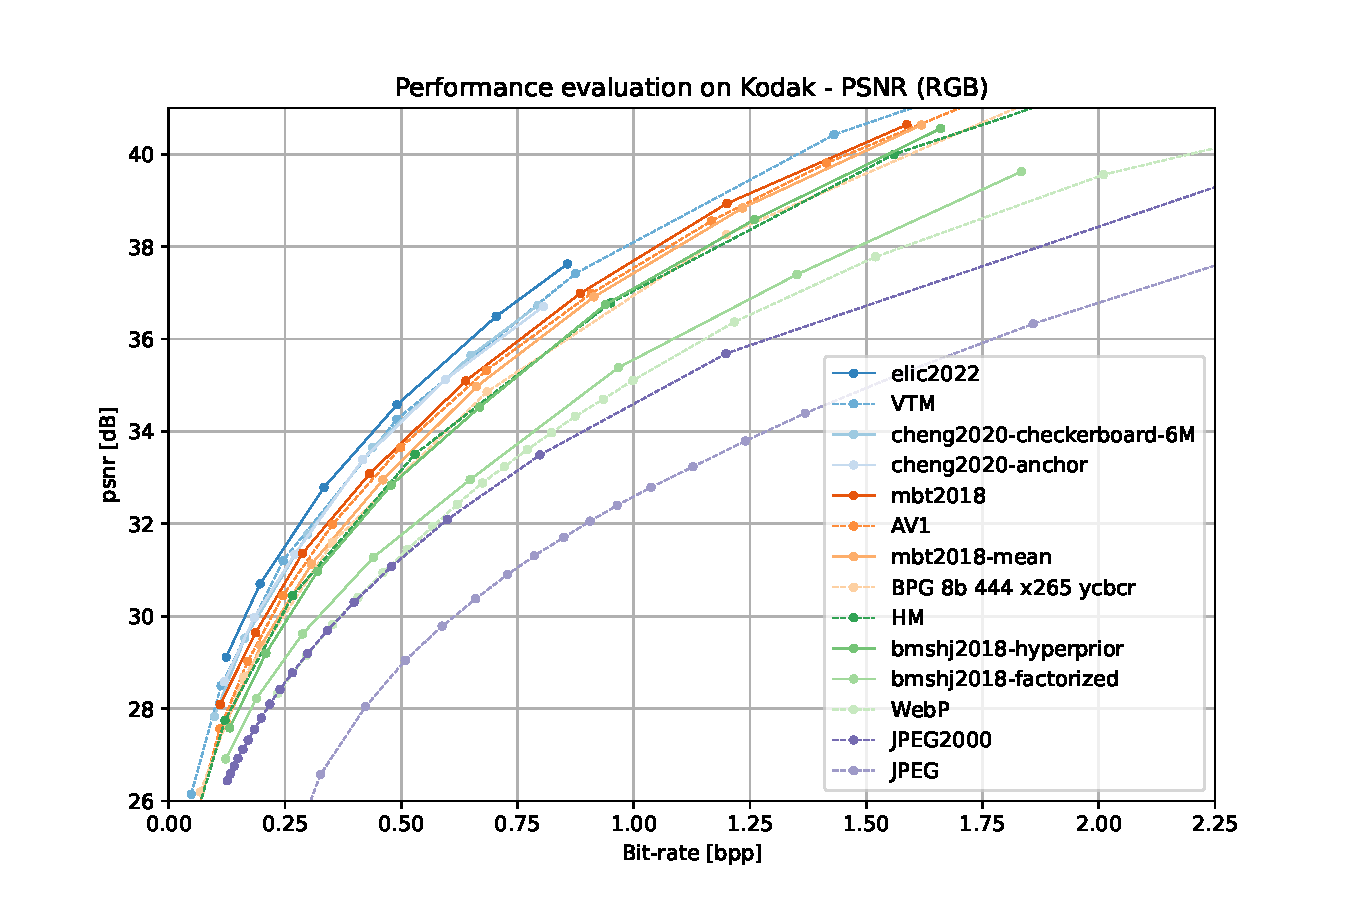
\includegraphics[width=\linewidth]{img/introduction/rd-curves-image-kodak-psnr-rgb.png}
  \caption[RD curves of all codecs on the Kodak dataset]{%
    RD curves for image compression codecs on the Kodak dataset~\cite{kodak_dataset}.%
    % PSNR vs. bitrate for various image compression codecs on the Kodak dataset.
  }
  \label{fig:intro/rd-curves}
\end{figure}

% Non-learned codecs are marked by dashed lines.
% Learning-based codecs offer further advantages by being easier to tune for targeted data sources, e.g. faces or screencasts.  % NEEDSCITATION

% These techniques can be applied to many types of data sources, including images, video, audio, and point clouds.
Learned compression has been applied to various types of data including images, video, and point clouds.
For learned image compression, most prominent are approaches based on Ballé~\emph{et~al.}'s compressive variational autoencoder (VAE), including~\cite{minnen2018joint,cheng2020learned,he2022elic}.
Other approaches based on RNNs and GANs have also been applied, including~\cite{toderici2017rnn,mentzer2020highfidelity}.
Works in learned point cloud compression include~\cite{yan2019deep,he2022density,pang2022graspnet,fu2022octattention,you2022ipdae}, and works in learned video compression include~\cite{rippel2019learned,agustsson2020scalespaceflow,hu2021fvc,ho2022canf}.
% Ballé~\emph{et~al.}'s~\cite{balle2018variational} foundational work is introduced in more detail below in SECTION.

% Disadvantages: more computation, less interpretable
Currently, one factor inhibiting industry adoption of learning-based codecs is that they are much more computationally expensive than traditional codecs like JPEG and WebP.
In fact, learned compression codecs exceed reasonable computational budgets by a factor of 100--10000\texttimes{}.
To remedy this, there is work being done towards designing low-complexity codecs for image compression, including~\cite{galpin2023entropy,ladune2023coolchic,leguay2023lowcomplexity,kamisli2023lowcomplexity}.

% Edge devices. IoT.
Learned compression has also shown benefits when applied to learned machine or computer vision tasks.
In Coding for Machines (CfM) --- also referred to as Video Coding for Machines (VCM)~\cite{duan2020vcm} --- compression is used for machine tasks such as classification, object detection, and semantic segmentation.
In this paradigm, the encoder-side device compresses the input into a compact task-specialized bitstream that is transmitted to the decoder-side device or server for further inference.
This idea of partially processing the input allows for significantly lower bitrates in comparison to transmitting the entire unspecialized input for inference.
Extending this technique, scalable multi-task codecs such as~\cite{choi2021latentspace,choi2022sichm} allocate a small base bitstream for machine tasks, and a larger enhancement bitstream for a higher-quality input reconstruction intended for human viewing.




\section{Compression architecture overview}

A simple compression architecture used by both traditional and learned compression methods alike is shown in \cref{fig:intro/arch-comparison/factorized}.
This architecture consists of several components.
\cref{tbl:intro/codec_components} lists some common choices for the components in this architecture.

\begin{figure}[htbp]
  \centering
  \begin{subfigure}{0.8\linewidth}
    \centering
    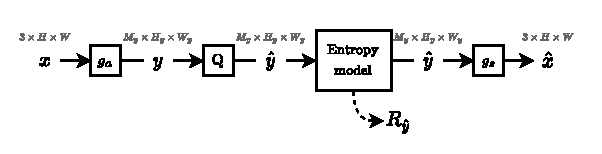
\includegraphics[width=\linewidth]{img/introduction/arch-overview-factorized.png}
    \caption{simple}
    \label{fig:intro/arch-comparison/factorized}
  \end{subfigure}%
  \par
  % \vspace{1.5\baselineskip}
  \begin{subfigure}{0.8\linewidth}
    \centering
    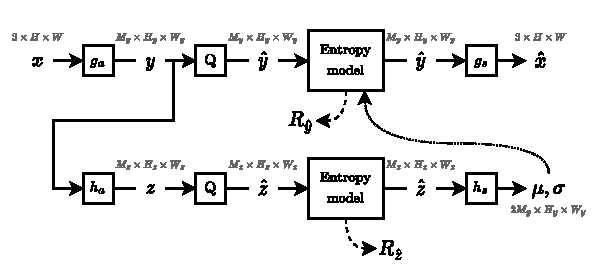
\includegraphics[width=\linewidth]{img/introduction/arch-overview-hyperprior.png}
    \caption{hyperprior}
    \label{fig:intro/arch-comparison/hyperprior}
  \end{subfigure}%
  \caption[High-level comparison of codec architectures]{%
    High-level comparison of codec architectures.%
  }
  \label{fig:intro/arch-comparison}
\end{figure}


\begin{table}[htbp]
  \centering
  \caption[Compression architecture overview for image codecs]{%
    Components of a compression architecture for various image compression codecs.%
  }
  \label{tbl:intro/codec_components}
  \footnotesize
  \def\arraystretch{2.5}
  \begin{tabular}[]{ccccc}
    \toprule
    \thead{Model}
      & \thead{Quantizer}
      & \thead{Entropy coding}
      & \thead{Analysis transform \\ ($g_a$)}
      & \thead{Synthesis transform \\ ($g_s$)}
      \\
    \midrule
    JPEG
      & non-uniform
      & \makecell{zigzag + RLE, \\ Huffman}
      & $8 \times 8$ block DCT
      & $8 \times 8$ block DCT$^{-1}$
      \\
    JPEG 2000
      & \makecell{uniform dead-zone \\ or trellis coded (TCQ)}
      & arithmetic
      & multilevel DWT
      & multilevel DWT$^{-1}$
      \\
    bmshj2018-factorized
      & uniform
      & arithmetic
      & (Conv, GDN) $\times 4$
      & (ConvT, IGDN) $\times 4$
      \\
    \bottomrule
  \end{tabular}
\end{table}


In this architecture, the input $\boldvar{x}$ goes through a transform $g_a$ to generate an intermediate representation $y$, which is quantized to $\boldvar{\hat{y}}$.
Then, $\boldvar{\hat{y}}$ is losslessly entropy coded to generate a transmittable bitstream from which $\boldvar{\hat{y}}$ can be perfectly reconstructed.
(at the decoder side.)
Finally, $\boldvar{\hat{y}}$ is fed into a synthesis transform $g_s$ which reconstructs an approximation of $\boldvar{x}$, which is labeled $\boldvar{\hat{x}}$.

Each of the components of the standard compression architecture are described in further detail below:
%
\begin{itemize}
  \item \textbf{Analysis transform} ($g_a$):
    The input first is transformed by the $g_a$ transform into a transformed representation $\boldvar{y}$.
    This transform often outputs a signal that contains less redundancy than within the input signal, and has its energy compacted into a smaller dimension.
    For instance, the JPEG codec transforms $8 \times 8$ blocks from the input image using a discrete cosine transform (DCT).
    This concentrates most of the signal energy into the low-frequency components that are often the dominating frequency component within natural images.
    In the case of learned compression, the analysis transform is often a nonlinear transform comprised of multiple deep layers and many parameters.
    For instance, the bmshj2018-factorized model's $g_a$ transform contains 4 downsampling convolutional layers interleaved with GDN~\cite{balle2016gdn} nonlinear activations, totaling 1.5M to 3.5M parameters.

  \item \textbf{Quantization}:
    The analysis transform outputs coefficients contained in a rather large (potentially even continuous) support.
    However, much of this precision is not necessary for a reasonably accurate reconstruction.
    Thus, we drop most of this unneeded information by binning the transformed coefficients into a much smaller discretized support.
    There are many choices for the reconstructed quantization bin values and boundaries.
    Popular quantizers include the uniform, dead-zone, Lloyd-Max, and Trellis-coded quantizers.
    % scalar and vector quantization
    Ballé~\emph{et~al.}~\cite{balle2018variational} use a uniform quantizer during inference, which is replaced with additive unit-width uniform noise during training.
    More recently, the STE quantizer has also been used during training.

  \item \textbf{Entropy coding}:
    The resulting $\boldvar{\hat{y}}$ is losslessly compressed using an entropy coding method.
    The entropy coder is targeted to match a specific encoding distribution.
    Whenever the encoding distribution correctly predicts an encoded symbol with high probability, the relative bit cost for encoding that symbol is reduced.
    Thus, some entropy models are context-adaptive, and change the encoding distribution on-the-fly in order to accurately probabilistically predict the next encoded symbol value.
    Huffman coding is used in JPEG, though it has trouble replicating a given target encoding probability distribution and also at adapting to dynamically changing encoding distributions.
    Thus, more recent codecs prefer to use arithmetic coders, which can much better approximate rapidly changing target encoding distributions.
    The CompressAI~\cite{begaint2020compressai} implementation uses rANS~\cite{duda2013asymmetric,giesen2014ryg_rans}, a popular recent innovation that is quite fast under certain conditions.

  \item \textbf{Synthesis transform} ($g_s$):
    Finally, the reconstructed quantized $\boldvar{\hat{y}}$ is fed into a synthesis transform $g_s$, which produces $\boldvar{\hat{x}}$.
    In JPEG, this is simply the inverse DCT.
    Similar to the analysis transform, in learned compression, the synthesis transform consists of several layers and many parameters.
    For instance, the bmshj2018-factorized model's $g_s$ transform contains 4 upsampling transposed convolutional layers interleaved with IGDN nonlinear activations, totaling 1.5M to 3.5M parameters.
\end{itemize}

The length of the bitstream is known as the rate cost $R_{\boldvar{\hat{y}}}$, which we seek to minimize. % in the task of compression
We also seek to minimize the distortion $D(\boldvar{x}, \boldvar{\hat{x}})$, which is typically the mean squared error (MSE) between $\boldvar{x}$ and $\boldvar{\hat{x}}$.
To balance these two competing goals, it is common to introduce a Lagrangian trade-off hyperparameter $\lambda$, so that the quantity sought to be minimized is $L = R_{\boldvar{\hat{y}}} + \lambda \, D(\boldvar{x}, \boldvar{\hat{x}})$.
% lossy, lossless: (lossy has non-zero D) (lossless has D = 0)


% TODO(table): parameters and MACs/pixel by model. Breakdown ga, gs, ha, hs, EP, CM, total.

% bmshj2018-factorized parameters and MACs/pixel:
%
% >>> N, M = 128, 192
% >>> sum([3 * N, N * N, N * N, N * M]) * 5**2 + sum([N**2, N**2, N**2])
% 1492352
% >>> sum([3 * N / 2**2, N * N / 4**2, N * N / 8**2, N * M / 16**2]) * 5**2
% 36800.0
%
% >>> N, M = 192, 320
% >>> sum([3 * N, N * N, N * N, N * M]) * 5**2 + sum([N**2, N**2, N**2])
% 3504192
% >>> sum([3 * N / 2**2, N * N / 4**2, N * N / 8**2, N * M / 16**2]) * 5**2
% 81600.0




\section{Entropy modeling}

A given element $\hat{y}_i \in \mathbb{Z}$ of the latent tensor $\boldvar{\hat{y}}$ is compressed using its encoding distribution $p_{{\hat{y}}_i} : \mathbb{Z} \to [0, 1]$, as visualized in \cref{fig:intro/encoding-distribution}.
The rate cost for encoding $\hat{y}_i$ is the negative log-likelihood, $R_{{\hat{y}}_i} = -\log p_{{\hat{y}}_i}({\hat{y}}_i)$, measured in bits.
Afterward, the exact same encoding distribution is used by the decoder to reconstruct the encoded symbol.
% (Thus, it is important to that the encoder and decoder are kept in sync.)
% The encoding distribution must be exactly the same at both the encoder and decoder, in exact synchronization.


\begin{figure}[htbp]
  \centering
  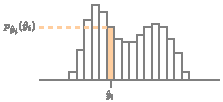
\includegraphics[width=0.8\linewidth]{img/introduction/encoding-distribution.png}
  \caption[Visualization of an encoding distribution for a single element]{%
    Visualization of an encoding distribution used for compressing a single element $\hat{y}_i$.%
  }
  \label{fig:intro/encoding-distribution}
\end{figure}


The encoding distributions are determined using an \emph{entropy model}.
\cref{fig:intro/encoding-distributions} visualizes the encoding distributions generated by well-known entropy models.
These are used to compress a latent tensor $\boldvar{\hat{y}}$ with dimensions $M_y \times H_y \times W_y$.
The exact total rate cost for encoding $\boldvar{\hat{y}}$ using $p_{\boldvar{\hat{y}}}$ is simply the sum of the negative log-likelihoods of each element, $R_{\boldvar{\hat{y}}} = \sum_i -\log p_{{\hat{y}}_i}({\hat{y}}_i)$.


\begin{figure}[htbp]
  \centering
  \begin{subfigure}[b]{0.5\linewidth}
    \centering
    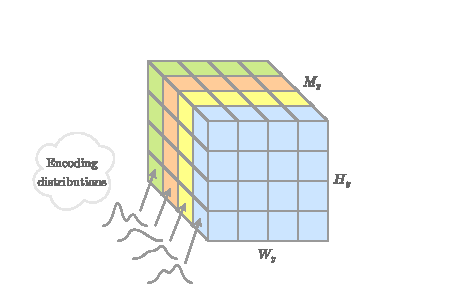
\includegraphics[width=\linewidth]{img/introduction/encoding-distributions-factorized.png}
    \caption{fully factorized}
    \label{fig:intro/encoding-distributions/factorized}
  \end{subfigure}%
  % \vspace{1.5\baselineskip}
  \begin{subfigure}[b]{0.5\linewidth}
    \centering
    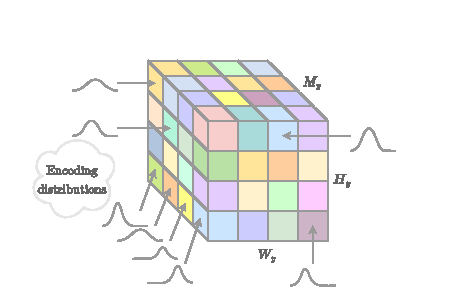
\includegraphics[width=\linewidth]{img/introduction/encoding-distributions-conditional.png}
    \caption{conditional}
    \label{fig:intro/encoding-distributions/conditional}
  \end{subfigure}%
  \caption[Visualization of encoding distributions for a latent tensor]{%
    Visualization of encoding distributions used for compressing a latent tensor $\boldvar{\hat{y}}$ with dimensions $M_y \times H_y \times W_y$.
    In (a), the encoding distributions within a given channel are all the same since the elements within a channel are assumed to be i.i.d. w.r.t. each other.
    Furthermore, in the case of the fully factorized entropy bottleneck used by Ballé~\emph{et~al.}~\cite{balle2018variational}, each encoding distribution is a static non-parametric distribution.
    In (b), the encoding distributions for each element are uniquely determined, and conditioned on side information.
    Furthermore, in the case of the Gaussian conditional hyperprior used by Ballé~\emph{et~al.}~\cite{balle2018variational}, the encoding distributions are Gaussian distributions parameterized by a mean and variance.%
  }
  \label{fig:intro/encoding-distributions}
\end{figure}


% TODO(review):  "Ballé~\emph{et~al.}~\cite{balle2018variational}" in full form is probably mentioned a bit too much here. Just the ~\cite{} is probably fine.

Some popular choices for entropy models include:
%
\begin{itemize}
  % Ballé~\emph{et~al.}~\cite{balle2017end} use a vector to parameterize a piecewise linear approximation of a continuous and differentiable density function f.

  \item
    A "fully factorized" \emph{entropy bottleneck}, as introduced by Ballé~\emph{et~al.}~\cite{balle2018variational}.
    Let $p_{{\hat{y}}_{c,i}} : \mathbb{Z} \to [0, 1]$ denote the probability mass distribution used to encode the $i$-th element $\hat{y}_{c,i}$ from the $c$-th channel of $\boldvar{\hat{y}}$.
    The same encoding distribution $p_{{\hat{y}}_c}$ is used for all elements within the $c$-th channel, i.e., $p_{{\hat{y}}_{c,i}} = p_{{\hat{y}}_c}, \forall i$.
    This entropy model works best when all such elements $\hat{y}_{c,1}, \hat{y}_{c,2}, \ldots, \hat{y}_{c,N}$ are independently and identically distributed (i.i.d.).

    Ballé~\emph{et~al.}~\cite{balle2018variational} model the encoding distribution as a static non-parametric distribution that is computed as the binned area under a probability density function $f_{c} : \mathbb{R} \to \mathbb{R}$, with a corresponding cumulative distribution function $F_{c} : \mathbb{R} \to [0, 1]$.
    % (This \emph{density} distribution differs from the encoding distribution, which is a probability \emph{mass} distribution that is supported by the quantization bins.)
    % TODO(figure): of f, with area for y +/- 1/2 underneath...
    Then,
    \begin{equation}
      \label{eqn:p_y_c_integral}
      p_{\boldvar{\hat{y}}_c}(\hat{y}_{c,i})
      = \int_{-\frac{1}{2}}^{\frac{1}{2}} f(\hat{y}_{c,i} + \tau) \, d\tau
      = F_{c}(\hat{y}_{c,i} + 1/2) - F_{c}(\hat{y}_{c,i} - 1/2).
    \end{equation}
    $F_{c}$ is modelled using a small fully-connected network composed of five linear layers with channels of sizes $[1, 3, 3, 3, 3, 1]$, whose parameters are tuned during training.
    Note that $F_{c}$ is not conditioned on any other information, and is thus static.

  \item
    A \emph{Gaussian conditional}, as introduced by Ballé~\emph{et~al.}~\cite{balle2018variational}.
    Let $f_i(y) = \mathcal{N}(y; {\mu_i}, {\sigma_i}^2)$ be a Gaussian distribution with mean ${\mu_i}$ and variance ${\sigma_i}^2$.
    Then, like in~\cref{eqn:p_y_c_integral}, the encoding distribution $p_{\boldvar{\hat{y}}_i}$ is the binned area under $f_i$:
    \begin{equation}
      \label{eqn:p_y_i_integral}
      p_{\boldvar{\hat{y}}_i}(\hat{y}_i)
      = \int_{-\frac{1}{2}}^{\frac{1}{2}} f_i(\hat{y}_i + \tau) \, d\tau.
      % = F_i(\hat{y}_i + 1/2) - F_i(\hat{y}_i - 1/2).
    \end{equation}
    In the mean-scale variant of the "hyperprior" model introduced by Ballé~\emph{et~al.}~\cite{balle2018variational},
    the parameters ${\mu_i}$ and ${\sigma_i}^2$ are computed by
    $[{\mu_i}, {\sigma_i}^2] = (h_s(\boldvar{\hat{z}}))_i$.
    Here, the latent representation $\boldvar{\hat{z}} = \operatorname{Quantize}[h_a(\boldvar{y})]$ is computed by the analysis transform $h_a$, and then encoded using an entropy bottleneck and transmitted as \emph{side information};
    and $h_s$ is a synthesis transform.
    This architecture is visualized in \cref{fig:intro/arch-comparison/hyperprior}.
    Cheng~\emph{et~al.}~\cite{cheng2020learned} define $f_i$ as a mixture of $K$ Gaussians --- known as a Gaussian mixture model (GMM) --- with parameters ${\mu}_{i}^{(k)}$ and ${\sigma}_{i}^{(k)}$ for each Gaussian, alongside an affine combination of weights ${w}_{i}^{(1)}, \ldots, {w}_{i}^{(K)}$ that satisfy the constraint $\sum_k {w}_{i}^{(k)} = 1$.
    A GMM encoding distribution is thus defined as
    $f_i(y) = \sum_{k=1}^{K} {w}_{i}^{(k)} \, \mathcal{N}(y; {\mu}_{i}^{(k)}, ({\sigma}_{i}^{(k)})^2)$.
\end{itemize}




\section{Thesis outline and contributions}

% Literary reference to "A silence of three parts"?
This thesis presents three main contributions:
%
\begin{itemize}
  \item
    In \cref{ch:pdf_compression}, "\nameref{ch:pdf_compression}",
    we present a method that can dynamically adapt the encoding distribution to the latent data distribution of a specific input.
    It does so by compressing and transmitting the distribution as side information.
    This is done using a small learned compression model that is specialized for compressing the encoding distributions.
    In comparison to competing methods such as a scale hyperprior, our method requires 25--130\texttimes{} less computation.
    % Furthermore, our method can also be used on top of existing entropy models as an encoding distribution correction method.
  \item
    In \cref{ch:point_cloud_compression}, "\nameref{ch:point_cloud_compression}",
    we present a PointNet-based point cloud codec that is specialized for classification.
    Our codec attains a 94\% reduction in BD-bitrate over non-specialized codecs on the ModelNet40 dataset.
    We also provide very lightweight model configurations of our codec that achieve similar bitrate improvements but with a very low computational cost.
  \item
    In \cref{ch:video_latent_space_motion_analysis}, "\nameref{ch:video_latent_space_motion_analysis}",
    we analyze how motion between consecutive input image frames $x_1$ and $x_2$ affects the corresponding latent representations $y_1$ and $y_2$ of typical convolutional neural networks (CNNs).
    Specifically, given a known optical motion between $x_1$ and $x_2$, we quantify how well $y_2$ can be predicted by applying that same motion to $y_1$.
    Since learned video compression models encode convolutionally-derived latent representations, it is useful to know how predictably or naturally the latent space behaves under input motion.
\end{itemize}




\subsection*{Publications and work during MASc}
% \subsection*{Contributions during MASc}
% \subsection*{Conference papers, demos, and software}


\subsubsection*{Used within this thesis}

\begin{enumerate}
  \item \fullciteall{ulhaq2023pointcloud}
  \item \fullciteall{ulhaq2021analysis}
\end{enumerate}


\subsubsection*{Other contributions}

\begin{enumerate}[resume]
  \item \fullciteall{ozyilkan2023learned}
  \item \fullciteall{ulhaq2022compressaitrainer}
  \item \fullciteall{choi2022frequencyaware}
  \item \fullciteall{alvar2022joint}
  \item \fullciteall{ulhaq2020colliflow}
\end{enumerate}


% \subsection*{Publications and work during BASc}
%
% \begin{enumerate}[resume]
%   \item \fullciteall{ulhaq2020thesisbasc}
%   \item \fullciteall{ulhaq2019neurips_demo}
% \end{enumerate}




% Other possible topics to introduce (not necessarily needed):
%
% Compression (briefly: Shannon, lossy, lossless, arithmetic coding)
% VAEs (briefly)
% Advanced learned entropy models: Cheng, ELIC, ...
